\chapter{Nombre del Capítulo 3} \label{chap:3}

Este capítulo tiene como objetivo, describir la propuesta para la transformación de los datos existentes en bases de datos conocidas, en datos que se gestionan en la herramienta TEAMSOFT$^+$. Para lograr esto, se muestran los artefactos de ingeniería de software necesarios, para entender su funcionamiento, como son: diagrama de casos de uso del sistema, requisitos funcionales y no funcionales. Para finalizar el capítulo se describe la validación de la funcionalidad presentada. Para esto, se realiza un mapeo entre las tablas de la base de datos utilizadas en dicho sistema, y las tablas que utiliza TEAMSOFT$^+$.

%\vspace{0.5cm}
%
%\section{Características de la herramienta}
%
%
%\paragraph{Requisitos funcionales}
%\begin{itemize}
%	\item La aplicación debe permitir importar la información de los problemas de béisbol y docentes, almacenada en ficheros externos.
%	\item La aplicación debe exportar la información gestionada de manera que TEAMSOFT$^+$ lo pueda incorporar para darle solución al problema.
%	\item Editar y visualizar la información importada de los ficheros externos que contienen la información almacenada de los profesores/peloteros.
%	\item Insertar los valores necesarios a cumplir por las personas en los roles, competencias.
%	\item Establecer las incompatibilidades entre los roles y entre las personas.
%\end{itemize}
%
%\paragraph{Requisitos no funcionales}
%\begin{itemize}
%	\item Los permisos de acceso al sistema podrán ser cambiados solamente por el administrador.
%	\item El sistema debe tomar el cuenta las categorías docentes y los tipos de actividades estipuladas en el reglamento docente.
%	\item El sistema debe tomar en cuenta las posiciones del juego establecida en el reglamento del béisbol.
%	\item El sistema debe proporcionar mensajes de error que sean informativos y orientados al usuario.
%	\item El sistema debe poseer una interfaz gráfica amigable.
%\end{itemize}
%
%En el sistema interactúan tres tipos de usuarios principales. En la Figura \ref{fig:cu-sistema} se observan estos usuarios, junto con sus respectivos casos de uso.
%
%\begin{figure}[H]
%	%	\centering
%	\hspace{-0.5cm}
%	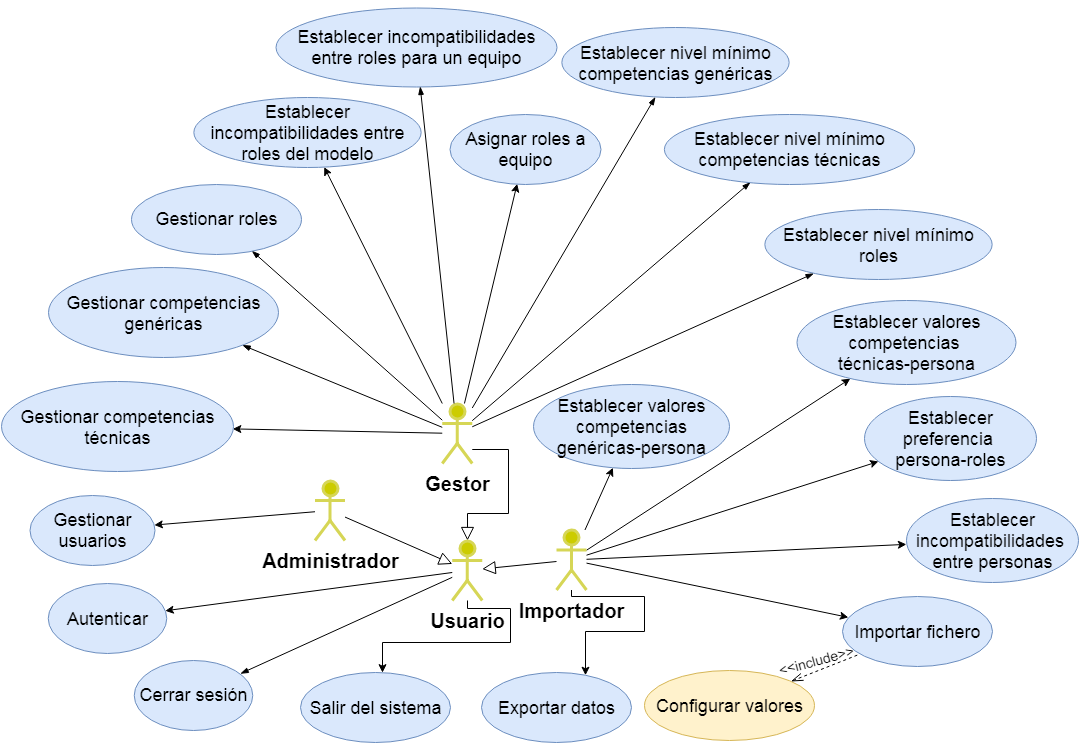
\includegraphics[width=1.1\textwidth]{figuras/DiagramaCUPP3.png}
%	\caption{Diagrama de caso de uso del sistema}\label{fig:cu-sistema}
%\end{figure}
%
%%\begin{table}[H]
%%	\centering
%En la Tabla \ref{desc-cu} se muestra para cada caso de uso presente en la Figura \ref{fig:cu-sistema}, la descripción detallada correspondiente.
%
%\begin{longtable}{| c | p{3cm} | p{9cm} |}
%	\caption{Descripción de los Casos de Uso}\label{desc-cu}\\
%	\toprule[1.7pt]
%	\textbf{No.} & \textbf{Caso de Uso} & \textbf{Descripción}\\ \hline
%	\endfirsthead
%	\multicolumn{3}{c}{\tablename - \thetable\ -- \textit{Continuación de la página anterior} }\\ \toprule[1.2pt]
%	\textbf{No.} & \textbf{Caso de Uso} & \textbf{Descripción}\\ \hline
%	\endhead
%	\multicolumn{3}{r}{\tablename - \thetable\ -- \textit{Continúa en la página siguiente} }\\
%	\endfoot
%	\endlastfoot
%	
%	
%	CU1&Autenticar & Para poder interactuar con el sistema todos los usuarios deben de autenticarse. Para esto, el usuario en cuestión debe introducir su nombre y contraseña. En función de la existencia del usuario y la correspondencia de la contraseña introducida con la almacenada, se permite que el usuario entre al sistema o, se le muestra un mensaje de error informando lo sucedido.\\ \hline
%	
%	CU2&Cerrar sesión & Una vez que el usuario se autentica puede cerrar la sesión de trabajo actual. El sistema lanza un mensaje de confirmación, y si el usuario reafirma su decisión entonces es redireccionado a la pantalla de inicio, donde debe de introducir sus credenciales.\\ \hline
%	
%	CU3&Salir del sistema & Una vez que el usuario se autentica tiene la opción de salir de la aplicación. El sistema lanza un mensaje de confirmación, y en caso de que el usuario reafirme su decisión, se cierra el sistema.\\ \hline
%	
%	CU4&Gestionar usuarios & Este caso de uso lo desencadena cualquier usuario que esté registrado como \textit{administrador}. En función de la decisión del administrador, puede añadir, editar y eliminar usuarios. En el caso de la adición de usuarios, el decisor deberá de elegir el tipo de problema al cuál pertenecerá el nuevo usuario, así como los roles de este.\\ \hline
%	
%	CU5&Gestionar competencias genéricas & El caso de uso inicia cuando un usuario registrado como \textit{gestor} requiere añadir o eliminar competencias genéricas. Si desea añadir alguna competencia, es necesario que rellene los datos correspondientes.\\ \hline
%	
%	CU6&Gestionar competencias técnicas & El caso de uso lo inicia cualquier usuario registrado con el rol de \textit{gestor} que requiera añadir o eliminar competencias técnicas. Si desea añadir alguna competencia, es necesario que rellene los datos correspondientes\\ \hline
%	
%	CU7&Gestionar roles & Cualquier usuario registrado en el sistema bajo el rol de \textit{gestor}, puede añadir, editar o borrar los roles vinculados al problema al que pertenece el usuario.\\ \hline
%	
%	CU8&Establecer incompatibilidades entre roles del modelo & En este caso de uso el usuario con el rol de \textbf{gestor}, define las incompatibilidades entre los roles para todos los equipos pertenecientes a un problema (si estas existen). \\ \hline
%	
%	CU9&Establecer incompatibilidades entre roles para un equipo & Los usuarios registrados con el rol de \textbf{gestor} son los encargados de establecer para cada equipo, específicamente los roles que son incompatibles.\\ \hline
%	
%	CU10&Asignar roles a equipo & El caso de uso inicia cuando el \textbf{gestor} decide definir los roles que se deben cubrir en cada equipo. Primero se debe de seleccionar el equipo y después en función de los roles existentes, ir añadiendo los que considere necesario. Todos los roles que cuando se hayan añadido se marquen como necesarios, van a estar presentes en todos los equipos.\\ \hline
%	
%	CU11&Establecer nivel mínimo de competencia genérica & Los usuarios registrados en el sistema bajo el rol de \textbf{gestor} son los encargados de iniciar este caso de uso. Por defecto, el nivel mínimo a cumplir por una persona en una competencia genérica es 0. El usuario en cuestión, tiene la posibilidad de editar este valor para las todas las competencias genéricas.\\ \hline
%	
%	CU12&Establecer nivel mínimo de competencia técnica & Los usuarios registrados en el sistema bajo el rol de \textbf{gestor} son los encargados de iniciar este caso de uso. Por defecto, el nivel mínimo a cumplir por una persona en una competencia técnica es 0. El usuario en cuestión, tiene la posibilidad de editar este valor para las todas las competencias técnicas.\\ \hline
%	
%	CU13&Establecer nivel mínimo de preferencia de las personas por los roles & Los usuarios registrados en el sistema bajo el rol de \textbf{gestor} son los encargados de iniciar este caso de uso. Por defecto, el nivel mínimo a cumplir por una persona en un rol es 0. El usuario en cuestión, tiene la posibilidad de editar este valor para las todas los roles.\\ \hline
%	
%	CU14&Importar fichero & Se inicia cuando se desea cargar la información de nuevas personas. El \textbf{importador} debe elegir el lugar donde se encuentra el fichero que constituye la fuente de datos. Después de seleccionado el fichero, en función del tipo de problema, debe de configurar las constantes que se tienen en cuenta en las ecuaciones para la transformación de los datos.
%	\\ \hline
%	
%	CU15&Exportar datos & Los usuarios que respondan al rol de \textbf{importador}, son los encargados de la exportación de los datos manejados en el sistema hasta el momento. Este usuario debe elegir los equipos y las personas que va a exportar. Estos datos, así como con los que se relacionan, se transforma e introducen en la base de datos de TEAMSOFT$^+$.\\ \hline
%	
%	CU16&Establecer valores de las competencias-genéricas & Este caso de uso se inicia después que se realizó el proceso de importación al menos una vez con éxito (existan personas importadas). Los usuarios registrados como \textbf{importador} son los encargados de establecer para cada persona, los valores de las competencias genéricas.\\ \hline
%	
%	CU17&Establecer valores de las competencias-técnicas & Este caso de uso se inicia después que se realizó el proceso de importación, al menos una vez con éxito (existan personas importadas). Los datos mostrados para cada persona son el resultado de las transformaciones pertinentes de los datos provenientes de los ficheros. Los usuarios registrados como \textbf{importador} son los encargados de editar, para cada persona, los valores de las competencias técnicas.\\ \hline
%	
%	CU18&Establecer preferencia persona-roles & Este caso de uso se inicia después que se realizó el proceso de importación, al menos una vez con éxito (existan personas importadas). Los datos mostrados para cada persona son el resultado de las transformaciones pertinentes de los datos provenientes de los ficheros. Los usuarios registrados como \textbf{importador} son los encargados de editar, para cada persona, los valores de preferencia por cada rol.\\ \hline
%	
%	CU19&Establecer incompatibilidades entre personas & Este caso de uso se inicia después que se realizó el proceso de importación, al menos una vez con éxito (existan personas importadas). Aquellos usuarios registrados bajo el rol de \textbf{importador} se encargan de asignar cuáles personas son incompatibles entre sí.\\
%	\bottomrule[1pt]
%\end{longtable}
%%	\end{tabular}
%%\end{table}
%
%En la Figura \ref{fig:pantalla-principal} se observa el prototipo para la interfaz de la herramienta propuesta, la cual garantiza el cumplimiento de los requisitos funcionales y no funcionales. Por ejemplo, el menú \textit{Usuario}, abarca del CU1 al CU4. En el menú \textit{Configuración problema} se gestionan los casos de uso del CU5 al CU14, mientras que en \textit{E/S} se garantizan del CU15 al CU19.
%
%\begin{figure}[H]
%	\centering
%	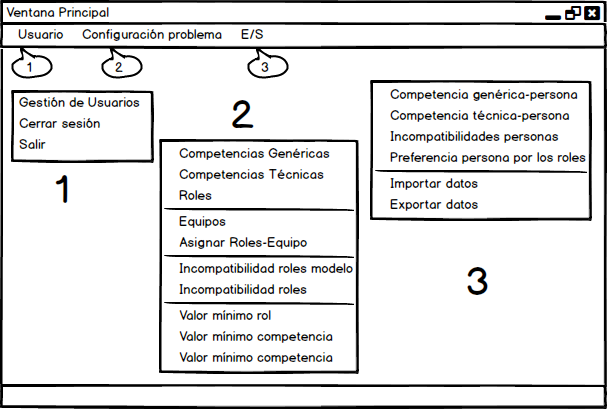
\includegraphics[width=1\textwidth]{figuras/VentanaPrincipal.png}
%	\caption{Ventana principal de la aplicación}\label{fig:pantalla-principal}
%\end{figure}
%
%
%En la Figura \ref{fig:diag-clases} se muestra el diagrama de clases utilizado para darle soporte al problema. Para su diseño se tuvieron en cuenta los siguientes aspectos:
%\begin{itemize}
%	\item En el diagrama se ha creado una clase para cada entidad simple del problema.
%	\item La relación de incompatibilidad entre las personas se modela mediante la relación de 0 a muchos entre la clase personas. El extremo 0 indica que una persona puede no tener incompatibilidad con otra persona.
%	\item La preferencia de las personas por los roles se muestra en la agregación entre las clases Persona y Rol.
%	\item La agregación entre Persona y Problema indica que una persona está disponible para ser asignado a un rol dentro de un equipo para un problema en particular.
%	\item Las relaciones de multiplicidad de muchos a muchos, que en el modelo relacional se representan a través de una tabla auxiliar asociativa, en el diagrama de clases solamente se muestran a través de una simple relación de agregación especificando la multiplicidad.
%\end{itemize}
%
%\begin{figure}[H]
%	\centering
%	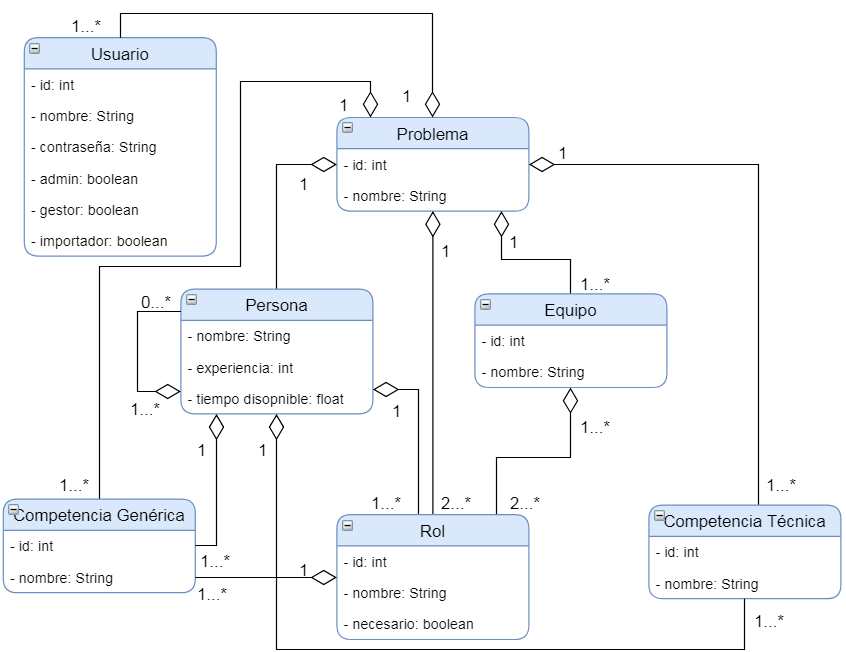
\includegraphics[width=1\textwidth]{figuras/diagramaClases.png}
%	\caption{Diagrama de clases}\label{fig:diag-clases}
%\end{figure}
%
%En la Figura \ref{fig:estruct-fichero} se muestra la estructura que tienen los ficheros a importar por el sistema para cada tipo de problema. El formato del fichero utilizado fue \textit{csv}, debido que es fácil de editar desde cualquier editor de texto y ocupa poco espacio. Cada fila del fichero almacena la información de una persona. Para cada persona se guardan además de sus estadísticas, la experiencia acumulada en cada rol. Puede verse un ejemplo en la Figura \ref{fig:ejemplo-estruct-fichero} (son los mismos datos utilizados para poblar las Tablas \ref{estadistica-of}, \ref{estadistica-def}, \ref{exp-of} y \ref{exp-def}).
%
%\begin{figure}[H]
%	\centering
%	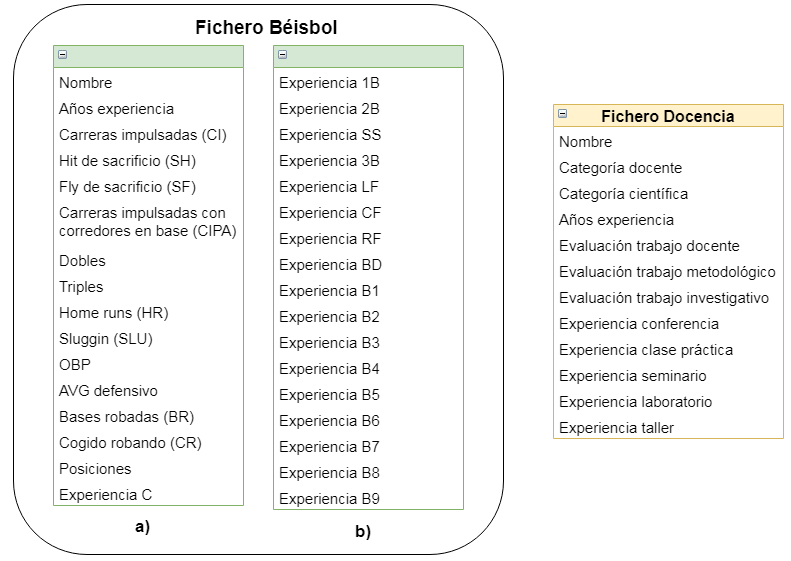
\includegraphics[width=1\textwidth]{figuras/estructuraFichero.png}
%	\caption{Estructura de los ficheros}\label{fig:estruct-fichero}
%\end{figure}
%
%\begin{figure}[H]
%	\centering
%	\subfigure[Fichero de béisbol \label{fig:fichero-beisbol}]{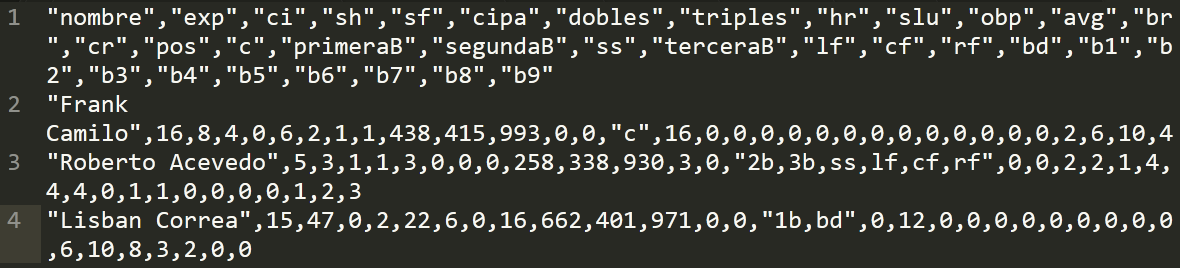
\includegraphics[width=1\textwidth]{figuras/ejemploFicheroPelota.png}}
%	\subfigure[Fichero de docencia \label{fig:fichero-docencia}]{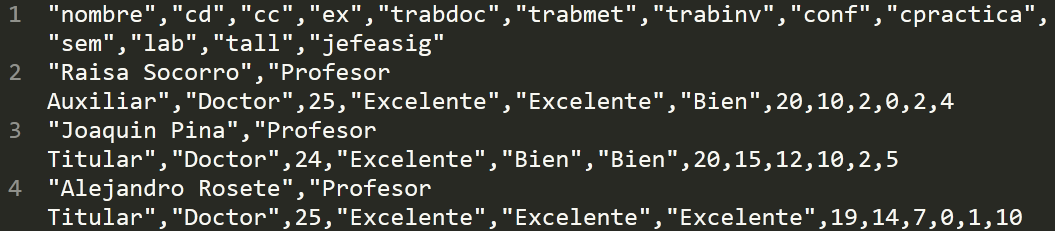
\includegraphics[width=1\textwidth]{figuras/ejemploFicheroDocente.png}}
%	
%	\caption{Estructura de los ficheros}\label{fig:ejemplo-estruct-fichero}
%\end{figure}
%
%\section{Validación de la herramienta}
%
%La herramienta desarrollada en este trabajo gestiona la información pertinente a los problemas de conformación de equipos de béisbol y docencia. Además, el proceso de exportación crea un puente entre los datos, y la posibilidad de conformar equipos con TEAMSOFT$^+$. En esta sección se comprueba el correcto funcionamiento de la herramienta a través de los procesos de importación y exportación, casos de usos CU14 y CU15 descritos en la Tabla \ref{desc-cu}.
%
%\subsection{Importación de los datos}
%
%El usuario que responde al rol de importador debe elegir el lugar donde se encuentra el fichero que constituye la fuente de datos para el tipo de problema. Además, debe de configurar las constantes que se tienen en cuenta en las ecuaciones para la transformación de los datos. En la Figura \ref{fig:conf-constantes} se pueden ver los valores de las constantes utilizadas durante el proceso de importación. El resultado de este proceso, permite obtener de forma automática el grado de preferencia de las personas por los roles, y el valor que tienen las personas en cada una de las competencias técnicas asociadas al problema. \\
%
%\begin{figure} [H]
%	\centering
%	\subfigure[\label{e}]{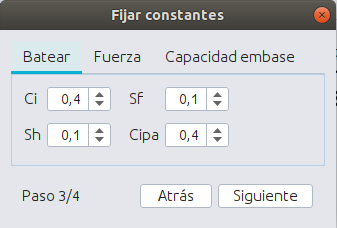
\includegraphics[width=0.45\textwidth]{figuras/fijarConstantes1.png}}
%	\subfigure[\label{s}]{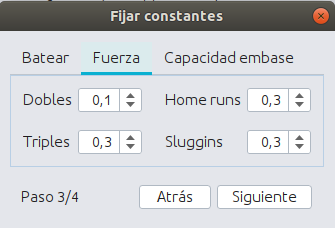
\includegraphics[width=0.45\textwidth]{figuras/fijarConstantes2.png}}
%	\subfigure[\label{f}]{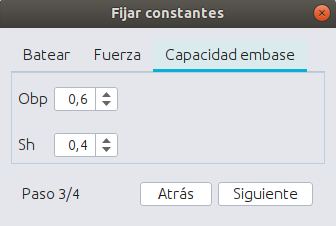
\includegraphics[width=0.45\textwidth]{figuras/fijarConstantes3.png}}
%	
%	\caption{Configuración de las constantes durante el proceso de importación} \label{fig:conf-constantes}
%\end{figure}
%
%Tomando como ejemplo los datos provenientes del fichero de béisbol, mostrados en la Figura \ref{fig:fichero-beisbol} y las constantes que se observan en la Figura \ref{fig:conf-constantes}, se obtienen como resultado los datos mostrados en la Figura \ref{fig:import-comp-tec}. Los datos resultantes y la información mostrada en las Tablas \ref{transf-pel}, \ref{pref-rol-of-pel} y \ref{pref-rol-def-pel} son calculados con las mismas constantes. A simple vista se pueden observar que son iguales. Se puede llegar a la conclusión entonces, que el proceso de importación funciona correctamente. 
%
%\begin{figure} [H]
%	\centering
%	\subfigure[Experiencia de los jugadores]{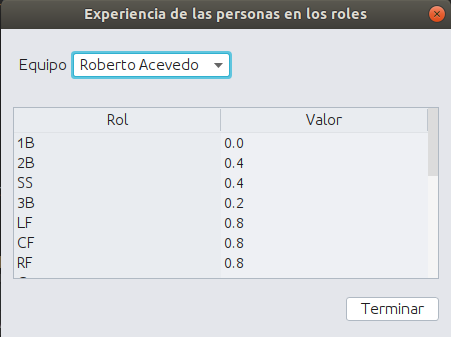
\includegraphics[width=0.6\textwidth]{figuras/importarExpEval.png}}
%	\subfigure[Competencias técnicas de los jugadores]{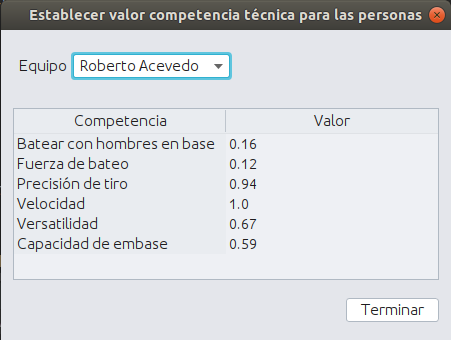
\includegraphics[width=0.6\textwidth]{figuras/importarCompTecEval.png}}
%	
%	\caption{Resultado de la importación para el problema de béisbol} \label{fig:import-comp-tec}
%\end{figure}
%
%\subsection{Exportación de los datos}
%
%El proceso de exportación de los datos consta de cuatro grandes pasos (ver Figura \ref{fig:proceso-export}). El usuario que responde al rol importador es el encargado de cada uno de ellos. El primer paso es donde se eligen los equipos a solucionar (ver Figura \ref{fig:equipos-exportar}). El siguiente se encarga de elegir las personas de interés para formar parte de los equipos seleccionados (ver Figura \ref{fig:personas-exportar}).
%
%\begin{figure}[H]
%	\centering
%	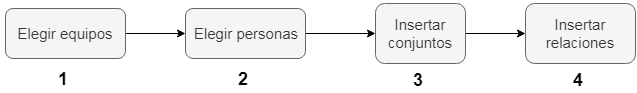
\includegraphics[width=1\textwidth]{figuras/flujoExport.png}
%	\caption{Proceso de exportación de los datos}\label{fig:proceso-export}
%\end{figure} 
%
%\begin{figure}[H]
%	\centering
%	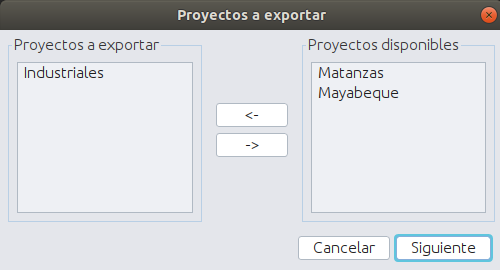
\includegraphics[width=0.6\textwidth]{figuras/exportarEquipo.png}
%	\caption{Ventana para elegir los equipos a exportar}\label{fig:equipos-exportar}
%\end{figure}   
%
%\begin{figure}[H]
%	\centering
%	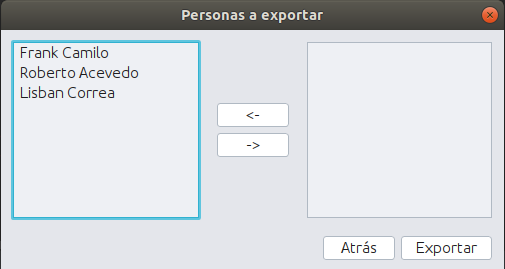
\includegraphics[width=0.6\textwidth]{figuras/exportarPersonas.png}
%	\caption{Ventana para elegir las personas a exportar}\label{fig:personas-exportar}
%\end{figure}   
%
%Después que fuesen elegidos los equipos y las personas, se insertan todos los conjuntos que se relacionan con ellos, y a su vez, las relaciones que existen entre esos conjuntos. Este proceso se realiza de esta forma debido a la dependencia existente los datos.
% 
%\subsubsection{Descripción de las tablas de TEAMSOFT$^+$}
%Como parte de este trabajo se desarrolla un sistema que permite la transformación de datos que almacenan información de las personas y se encuentran en ficheros externos, en datos entendibles por el sistema TEAMSOFT$^+$. Los valores de competencia y preferencia de las personas asignados a estas, resultan objetivo, partiendo que se obtienen de datos almacenados en sistemas, sitios o herramientas que constituyen la fuente de datos en cada uno de los problemas analizados en este trabajo. Una vez importada la información de las personas y realizadas las transformaciones pertinentes en cada caso, es necesario exportar la información hacia la base de datos con la que trabaja el sistema TEAMSOFT$^+$ para su solución posterior. En la Figura \ref{fig:tablas-teamsoft} se muestran todas las tablas de la base de datos utilizadas en la exportación por la herramienta desarrollada como parte de este trabajo. Marcadas en un rectángulo rojo, están aquellas en las que se realiza inserción de datos. A continuación se realiza una breve explicación de cada una de ellas:
%
%\begin{description}
%	\item[competence:] tabla donde se guardan todas las competencias, ya sean técnicas o genéricas. 
%	
%	\item[competence\_dimension:] esta tabla almacena una descripción para cada competencia, además de registrar el nivel en que se necesita.
%	
%	\item[competence\_importance:] tabla que almacena la importancia de cada competencia.
%	
%	\item[competence\_value:] almacena para cada persona, el nivel que posee en cada competencia.
%	
%	\item[conflict\_index:] tabla donde se registra el índice de conflicto entre las personas.
%	
%	\item[cycle:] almacena la estructura, fecha inicio y fecha fin de cada proyecto.
%	
%	\item[incompatible\_roles:]  guarda los roles incompatibles en todos los proyectos.
%	
%	\item[levels:] tabla donde se configura los niveles que tienen las competencias. 
%	
%	\item[person\_group:] almacena los grupos a los que pertenecen las personas. Existe una jerarquía de grupos, donde un grupo puede ser padre de otro, y por tanto, hereda sus personas.
%	
%	\item[personal\_interest:] almacena las preferencias de las personas por los roles.
%	
%	\item[project:] tabla donde se guardan todos los proyectos.
%	
%	\item[project\_role\_incomp:] registra todos los roles incompatibles por proyecto.
%	
%	\item[project\_roles:] tabla que almacena los roles necesarios en cada proyecto, así como la carga y el número de personas necesarias para desempeñarlos. 
%	
%	\item[project\_structure:] se registra la estructura de los proyectos.
%	
%	\item[project\_tech\_competence:] en cada proyecto, para cada rol, se registran las 
%	competencias técnicas necesarias, así como el nivel en que se necesitan y la importancia que posee. 
%	
%	\item[role:] se almacenan todos los roles.
%	
%	\item[role\_competition:] para cada rol, se almacena la importancia y nivel en que se necesitan las competencias genéricas.
%	
%	\item[role\_experience:] experiencia de los trabajadores en los roles
%	
%	\item[role\_load:] carga qu representa ocupar un rol. Esta tabla no es utilizada por el problema de la pelota debido a que no influye el tiempo.
%	
%	\item[work:] tabla donde se almacenan las personas.
%	
%	\item[work\_conflict:] se registran las incompatibilidades entre las personas.
%\end{description}
%
%\begin{figure}[H]
%	\centering
%	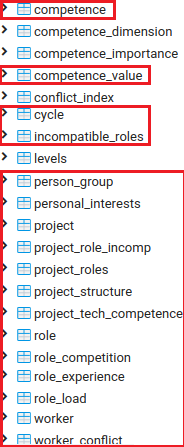
\includegraphics[width=0.23\textwidth]{figuras/tablasTeamSoft.png}
%	\caption{Tablas utilizadas de la base de datos de TEAMSOFT$^+$}\label{fig:tablas-teamsoft}
%\end{figure}
%
%\subsubsection{Mapeo de los datos}
%Para validar el correcto funcionamiento de la herramienta, resulta necesario conocer qué información de la gestionada, es necesario exportar a TEAMSOFT$^+$, y en qué tabla de la base de datos de este, se almacena. En caso de no existir un mapeo directo entre ambas bases de datos,  debe realizarse una transformación.\\
%
%Como parte del tercer paso de la Figura \ref{fig:proceso-export} se procede a la inserción de los conjuntos en la base de datos de TEAMSOFT$^+$. Como primer paso dentro de este, se insertan todos los equipos elegidos en la tabla \textbf{project}. TEAMSOFT$^+$ organiza a las personas a través de grupos. A la hora de exportar las personas hacia TEAMSOFT$^+$, es necesario que siga este formato. Para lograr esto se crea un nuevo grupo en la tabla \textbf{person\_group}, y todas las personas elegidas se insertan en la tabla \textbf{worker} asociadas al nuevo grupo. Después se procede a la inserción de los roles pertenecientes a los proyectos seleccionados en la tabla \textbf{role}. Quedando este proceso como se observa en la Figura \ref{fig:insert-equipo-y-personas}.
%
%\begin{figure}[H]
%	\centering
%	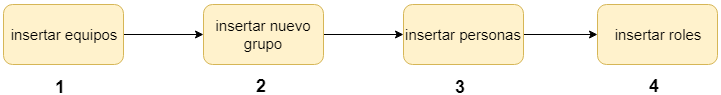
\includegraphics[width=0.8\textwidth]{figuras/insertEquipoPersonas.png}
%	\caption{Insertar equipos y personas}\label{fig:insert-equipo-y-personas}
%\end{figure}
%
%El diseño de la base de datos implementado en la herramienta, mantiene por separado las competencias técnicas de las genéricas. Mientras que en la base de datos de TEAMSOFT$^+$ se gestionan en una sola tabla. Se garantiza la distinción entre ellas, utilizando el campo booleano \textit{technical}. Cuando se realiza la exportación, todas las competencias, tanto técnicas como genéricas, se insertan en la tabla \text{competence}. Para el caso de las competencias técnicas, el valor del campo booleano sería verdadero, y falso para las genéricas.
%
%Una vez finalizado el tercer paso de la Figura \ref{fig:proceso-export}, se procede insertar todos los datos de las relaciones existentes entre los conjuntos exportados. Primeramente, se insertan todos los roles pertenecientes a los equipos en la tabla \textbf{project\_role}. Para esto es necesario realizar un cambio. En la herramienta la carga de trabajo se gestiona en una escala de cero a uno, mientras que en la base de datos de TEAMSOFT$^+$ se maneja en una escala del uno al cuatro (tabla \textbf{role\_load}). Para lograr la transformación, se separa la escala del cero al uno en cuatro conjuntos de igual tamaño, en función de dónde le corresponda el valor, es la escala que toma en la base de datos de TEAMSOFT$^+$. Por ejemplo, si la carga del rol $r_1$ en el equipo $e_1$ fuese de 0.34, su valor, una vez transformado le corresponde 3 (Media). La Tabla \ref{table:transformacion-carga} refleja estas transformaciones.
%
%\begin{table}[H]
%	\centering
%	\caption{Transformación de los valores de la carga de los roles}\label{table:transformacion-carga}
%	\begin{tabular}{c | c | c}
%		\toprule[1.7pt]
%		Valores de la Herramienta & Valores TEAMSOFT$^+$ & Descripción               \\ \midrule
%		        0.0 - 0.25          & 4                    & Baja                      \\ 
%		        0.26 - 0.50         & 3                    & Media                     \\ 
%		        0.51 - 0.75         & 2                    & Alta                      \\ 
%		        0.76 - 1.0          & 1                    & Muy alta \\ \bottomrule[1.1pt]
%	\end{tabular}
%\end{table}
%
%Una vez insertado los roles a los equipos, se inserta entonces, las incompatibilidades entre los roles en los equipos. Esto se realiza en la tabla \textbf{project\_role\_incom}. El siguiente paso sería entonces, insertar el valor que se necesita para cada competencia técnica en los roles de los proyectos en la tabla \textbf{project\_tech\_competence}. En este paso hay que realizar algunas transformaciones. Esta tabla gestiona la importancia para cada competencia, además del nivel que se necesita en ese rol para poder desempeñarlas. Al no gestionarse la importancia de las competencias en la herramienta, se mantiene fijo el valor en el nivel más bajo (alguna medida). El nivel necesario de las competencias se expresa en una escala del uno al cuatro, mientras que en la herramienta se gestiona de cero a uno. En la Tabla \ref{table:transformacion-nivel-competencia} se realiza el proceso de conversión.
%
%\begin{table}[H]
%	\centering
%	\caption{Transformación de los niveles de las competencias}\label{table:transformacion-nivel-competencia}
%	\begin{tabular}{c | c | c}
%		\toprule[1.7pt]
%		Valores de la Herramienta & Valores TEAMSOFT$^+$ & Descripción               \\ \midrule
%		0.0 - 0.25          & 1                    & en partida                      \\ 
%		0.26 - 0.50         & 2                    & en desarrollo                     \\ 
%		0.51 - 0.75         & 3                    & en avance               \\ 
%		0.76 - 1.0          & 4                    & experto \\ \bottomrule[1pt]
%	\end{tabular}
%\end{table}
%
%El siguiente paso sería insertar la relación entre las competencias genéricas y los roles en la tabla \textbf{role\_competition}. En esta tabla ocurre algo parecido a lo sucedido a la hora de exportar los datos de la tabla \textbf{project\_tech\_competence}, lo que esta vez no intervienen los equipos, solamente las competencias genéricas y los roles. La transformación sería la misma que se hizo en la Tabla \ref{table:transformacion-nivel-competencia}. También es necesario insertar las incompatibilidades entre los roles. Estas incompatibilidades son a nivel global, lo que significa en todos los equipos están presentes. Por ejemplo. El rol $r_1$ y el rol $r_2$ se definen como incompatibles en la tabla \textbf{incompatible\_roles}, estos roles serían incompatibles a su vez en todos los equipos.\\
%
%Lo siguiente sería insertar las relaciones donde intervienen las personas. La primera relación a insertar sería, las incompatibilidades entre la personas en la tabla \textbf{worker\_conflict}. Una vez realizada esta operación se procede a insertar las preferencias de las personas por los roles y la experiencia de las personas en los roles en las tablas \textbf{personal\_interest} y \textbf{role\_experience}, respectivamente. La herramienta desarrollada permite la obtención de la experiencia de las personas por los roles, teniendo en cuenta tiempo que llevan ejerciéndolos y el tiempo total de experiencia. En el caso de las preferencias de las personas por los roles, en la base de datos de TEAMSOFT$^+$ se gestiona como un valor booleano, si lo prefiere o no. Mientras que en la herramienta se trata en valores en la escala de cero a uno. El autor decide entonces, realizar un punto de corte en la escala. Todo valor que esté por encima de 0.5 se considera como si la persona tuviese preferencia por el rol. El proceso de exportación de los datos culmina con la inserción el valor de las personas en las competencias en la tabla \textbf{competence\_value}. Como ya se mencionaba anteriormente, en la herramienta se tratan por separado las competencias técnicas y genéricas. También se mencionó con anterioridad que los valores que le otorga la herramienta a las competencias oscila en la escala de cero a uno. Por lo tanto las transformaciones son las mismas que las presentadas en la Tabla \ref{table:transformacion-nivel-competencia}. La Figura \ref{fig:flujo-completo} muestra el diagrama de flujo que explica todo el proceso.
%
%\begin{figure}[H]
%	\centering
%	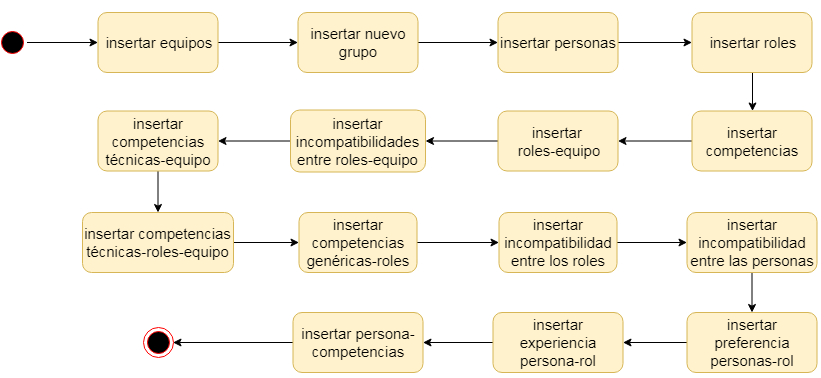
\includegraphics[width=0.9\textwidth]{figuras/flujoCompletoExport.png}
%	\caption{Diagrama de flujo del proceso de exportación}\label{fig:flujo-completo}
%\end{figure}
%
%Se comprueba el correcto funcionamiento del proceso de exportación si TEAMSOFT$^+$ carga exitosamente los datos exportados por la herramienta. En las Figuras \ref{fig:exportar-competencias}, \ref{fig:exportar-roles} y \ref{fig:exportar-personas} se muestran algunas capturas de pantalla de TEAMSOFT$^+$, una vez culminado el proceso de exportación.
%
%\begin{figure}[H]
%	\centering
%	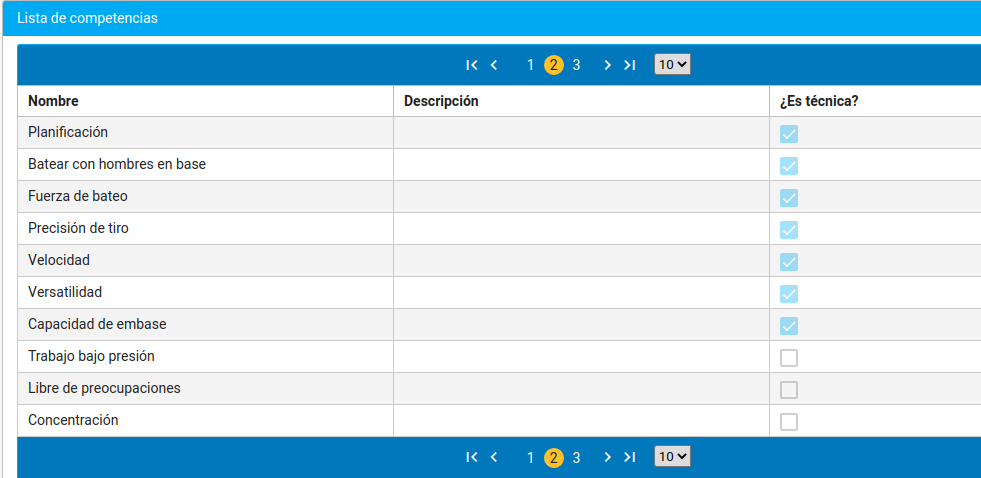
\includegraphics[width=0.9\textwidth]{figuras/exportarCompetencias.png}
%	\caption{Ventana para gestionar las competencias en TEAMSOFT$^+$}\label{fig:exportar-competencias}
%\end{figure}
%
%\begin{figure}[H]
%	\centering
%	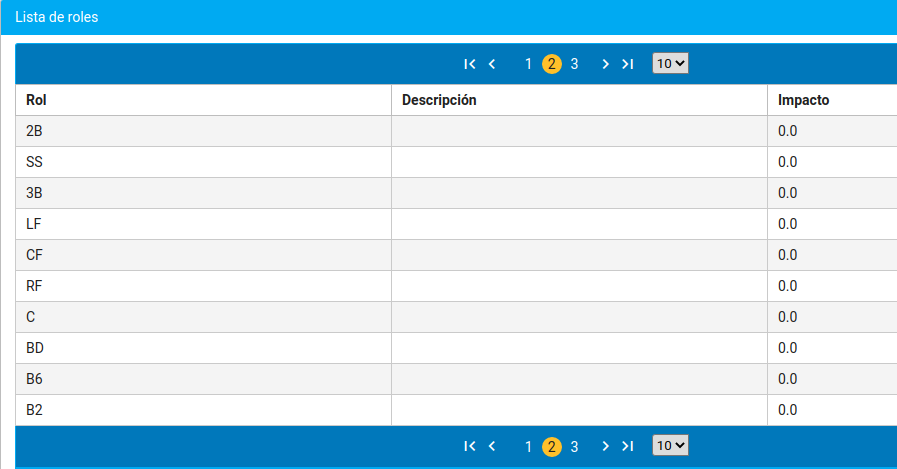
\includegraphics[width=0.9\textwidth]{figuras/exportarRoles.png}
%	\caption{Ventana para gestionar los roles en TEAMSOFT$^+$}\label{fig:exportar-roles}
%\end{figure}
%
%\begin{figure}[H]
%	\centering
%	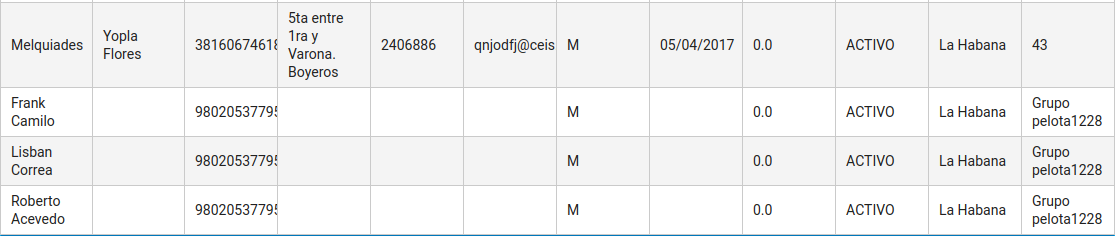
\includegraphics[width=1\textwidth]{figuras/exportarPersonasTeamsoft.png}
%	\caption{Ventana para gestionar las personas en TEAMSOFT$^+$}\label{fig:exportar-personas}
%\end{figure}
%
%\section{Conclusiones parciales}
%Con la terminación de este capítulo se llega a las siguientes conclusiones:
%\begin{enumerate}
%	\item Se implementó una herramienta para la obtención de las características de las personas para los problemas de conformación de equipos docentes y de béisbol, a partir de datos almacenados en sistemas, sitios o herramientas que constituyen la fuente de datos en cada uno de los problemas analizados en este trabajo.
%	\item Se validó que los datos exportados por la herramienta son leídos satisfactoriamente por TEAMSOFT$^+$.
%\end{enumerate}
